
\documentclass{abgabe}
\begin{document}

\begin{questions}
    \qformat{\thequestion. \textbf{\thequestiontitle} \hfill}
    \titledquestion{Boehm’sches Spiralmodell}
    In der Vorlesung wurde ein wichtiger Meilenstein bei der Entwicklung von Software-Entwicklungspro\-zessen ausgelassen, das so genannte Boehmsche Spiralmodell. 
    Informieren Sie sich über dieses Modell und beschreiben Sie die Hauptideen des Ansatzes. 
    Überlegen Sie, in wie weit es sich um ein iteratives Modell und dann um ein inkrementelles Modell handelt. 
    Dokumentieren Sie ihre Nachforschungen und Überlegungen.
    \begin{solution}
        \begin{center}
            \href{https://cdn1.vogel.de/unsafe/fit-in/1000x0/images.vogel.de/vogelonline/bdb/1363200/1363291/original.jpg}{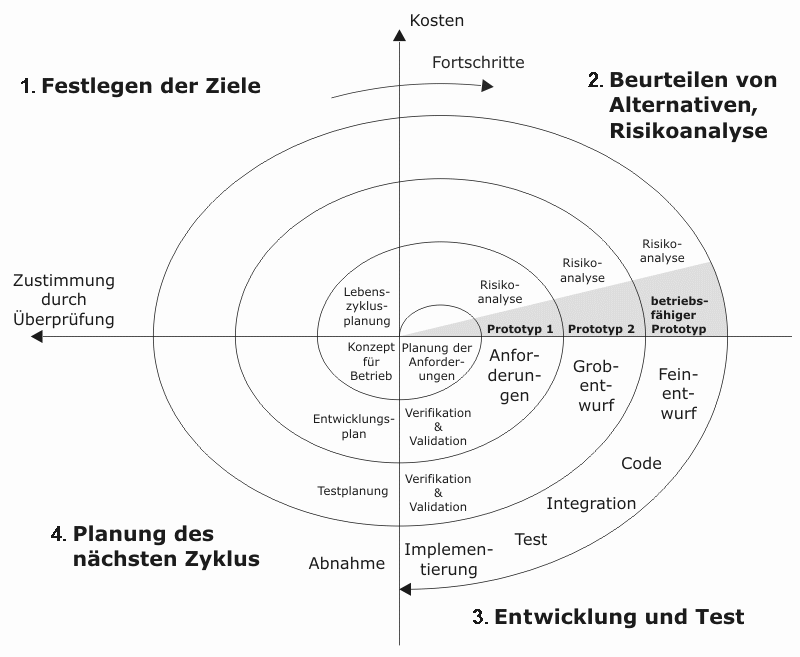
\includegraphics[width=1\textwidth]{Spiralmodel_nach_Boehm.png}}
            %\href{}{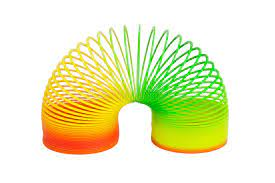
\includegraphics[width=1\textwidth]{spring.jpg}}
        \end{center}
        
        Von \href{https://www.dev-insider.de/was-ist-das-spiralmodell-a-692581/}{dev-insider}:
        
        \begin{displayquote}
            Der Entwicklungsprozess durchläuft die Spirale von innen nach außen. 
            Jede Umrundung stellt aufeinander aufbauende Phasen der Entwicklung dar. 
            Ein Entwicklungsprozess beginnt im Inneren der Spirale mit Risikoanalyse, grundlegender Konzeptentwicklung und der Bestimmung von Anforderungen.
            
            Der erste Quadrant bezieht sich jeweils auf die Ermittlung von Zielen, der zweite auf die Bewertung von Alternativen und die Reduktion von Risiken. 
            Im dritten Quadranten erfolgt die eigentliche Entwicklung, im Softwarebereich speziell die Implementierung. 
            Der vierte Quadrant leitet schließlich mit der Planung der nächsten Phasen wieder in den ersten über.
            
            Als Risiko-orientiertes Entwicklungsmodell bezieht das Spiralmodell die Risiken der Prozessabläufe wesentlich in die Ausgestaltung der Struktur ein. 
            Sie bestimmen sowohl den Grad der Detaillierung jeder einzelnen Stufe als auch, mit welchem Aufwand und Einsatz die jeweilige Stufe umzusetzen ist. 
            Eine Risikobewertung ist daher in jedem Umlauf im zweiten Quadranten vorgesehen.
            
            Allgemein fokussiert das Spiralmodell auf die langfristigen Einflüsse über den gesamten Lebenszyklus eines Produkts. 
            In Bezug auf Software bedeutet das vor allem ein Abrücken von einer zu starken Konzentration auf das Kodieren von Quelltext.
        \end{displayquote}
        
        Aus \href{https://de.wikipedia.org/wiki/Spiralmodell}{Wikipedia}: 
        \begin{displayquote}
            Das Spiralmodell gehört zu den inkrementellen oder iterativen Vorgehensmodellen. 
            Es ist eine Weiterentwicklung des Wasserfallmodells, in der die Phasen mehrfach spiralförmig durchlaufen werden.
            
            Das inkrementelle und iterative Vorgehensmodell sieht daher eine zyklische Wiederholung der einzelnen Phasen vor. 
            Dabei nähert sich das Projekt langsam den Zielen an, auch wenn sich die Ziele während des Projektfortschrittes verändern. 
            Durch das Spiralmodell wird nach Boehm das Risiko eines Scheiterns bei großen Softwareprojekten entscheidend verringert. 
        \end{displayquote}
        
        Meine Nachforschungen und Überlegungen sahen wie folgt aus:
        \begin{enumerate}
            \item \gqq{Boehm’sches Spiralmodell} googlen,
            \item den Wikipedia-Artikel öffnen
            \item um ihn dann wieder zu schließen,
            \item das zweite Google-Ergebnis einfach überspringen,
            \item im dritten Ergebnis eine fantastische Zusammenfassung finden und diese hier teilen!
            \item Bemerken, dass ich noch betrachten muss, in wie weit es sich um ein inkrementelles bzw. iteratives Modell handelt,
            \item den Wikipedia-Artikel erneut öffnen
            \item und die wunderbare Erläuterung hier hinzufügen!
        \end{enumerate}
    \end{solution}
\end{questions}
\end{document}